\documentclass[runningheads,a4paper]{llncs}

\usepackage[american]{babel}

\usepackage{graphicx}

%extended enumerate, such as \begin{compactenum}
\usepackage{paralist}

%put figures inside a text
%\usepackage{picins}
%use
%\piccaptioninside
%\piccaption{...}
%\parpic[r]{\includegraphics ...}
%Text...

%Sorts the citations in the brackets
%\usepackage{cite}

%for easy quotations: \enquote{text}
\usepackage{csquotes}

\usepackage[T1]{fontenc}

%enable margin kerning
\usepackage{microtype}

%better font, similar to the default springer font
\usepackage[%
rm={oldstyle=false,proportional=true},%
sf={oldstyle=false,proportional=true},%
tt={oldstyle=false,proportional=true,variable=true},%
qt=false%
]{cfr-lm}
%
%if more space is needed, exchange cfr-lm by mathptmx
%\usepackage{mathptmx}

\usepackage[
%pdfauthor={},
%pdfsubject={},
%pdftitle={},
%pdfkeywords={},
bookmarks=false,
breaklinks=true,
colorlinks=true,
linkcolor=black,
citecolor=black,
urlcolor=black,
%pdfstartpage=19,
pdfpagelayout=SinglePage
]{hyperref}
%enables correct jumping to figures when referencing
\usepackage[all]{hypcap}

\usepackage[capitalise,nameinlink]{cleveref}
%Nice formats for \cref
\crefname{section}{Sect.}{Sect.}
\Crefname{section}{Section}{Sections}
\crefname{figure}{Fig.}{Fig.}
\Crefname{figure}{Figure}{Figures}

\usepackage{xspace}
%\newcommand{\eg}{e.\,g.\xspace}
%\newcommand{\ie}{i.\,e.\xspace}
\newcommand{\eg}{e.\,g.,\ }
\newcommand{\ie}{i.\,e.,\ }

%introduce \powerset - hint by http://matheplanet.com/matheplanet/nuke/html/viewtopic.php?topic=136492&post_id=997377
\DeclareFontFamily{U}{MnSymbolC}{}
\DeclareSymbolFont{MnSyC}{U}{MnSymbolC}{m}{n}
\DeclareFontShape{U}{MnSymbolC}{m}{n}{
    <-6>  MnSymbolC5
   <6-7>  MnSymbolC6
   <7-8>  MnSymbolC7
   <8-9>  MnSymbolC8
   <9-10> MnSymbolC9
  <10-12> MnSymbolC10
  <12->   MnSymbolC12%
}{}
\DeclareMathSymbol{\powerset}{\mathord}{MnSyC}{180}

% correct bad hyphenation here
\hyphenation{op-tical net-works semi-conduc-tor}

\usepackage{listings}
\usepackage{color}

% java code highlighting
\definecolor{javared}{rgb}{0.6,0,0} % for strings
\definecolor{javagreen}{rgb}{0.25,0.5,0.35} % comments
\definecolor{javapurple}{rgb}{0.5,0,0.35} % keywords
\definecolor{javadocblue}{rgb}{0.25,0.35,0.75} % javadoc

\lstset{language=Java,
basicstyle=\small,%\ttfamily,
keywordstyle=\color{javapurple}\bfseries,
stringstyle=\color{javared},
commentstyle=\color{javagreen},
morecomment=[s][\color{javadocblue}]{/**}{*/},
numbers=left,
numberstyle=\tiny\color{black},
stepnumber=1,
numbersep=7pt,
tabsize=4,
showspaces=false,
showstringspaces=false}

\definecolor{darkgray}{rgb}{.4,.4,.4}

\lstdefinelanguage{AspectJ}[]{Java}{
    morekeywords={declare, pointcut, aspect, before, around, after, returning, throwing, call, execution, get, set, this, target, args, within, withincode, initialization, preinitialization, staticinitialization, handler, adviceexecution, cflow, cflowbelow, if, proceed},
    moredelim=[is][\textcolor{darkgray}]{\%\%}{\%\%},
    moredelim=[il][\textcolor{darkgray}]{§§}
}

\begin{document}

%Works on MiKTeX only
%hint by http://goemonx.blogspot.de/2012/01/pdflatex-ligaturen-und-copynpaste.html
%also http://tex.stackexchange.com/questions/4397/make-ligatures-in-linux-libertine-copyable-and-searchable
%This allows a copy'n'paste of the text from the paper
\input glyphtounicode.tex
\pdfgentounicode=1

\title{Fusing Loops of Collection Methods with AspectJ}
%If Title is too long, use \titlerunning
%\titlerunning{Short Title}

%Single insitute
\author{Nico Ring}
%If there are too many authors, use \authorrunning
%\authorrunning{First Author et al.}
\institute{Hasso Plattner Institute, University of Potsdam, Germany\\
\email{nico.ring@student.hpi.de}
}

\maketitle

\begin{abstract}
In this paper we present an approach to fuse loops of collection methods with an aspect-oriented solution\footnote{\url{https://github.com/nicoring/loopFusing}}.
With anonymous functions it is possible to create high-order methods like map or filter. These can be combined and reused in contrast to for-loops.
One problem with collection methods is that every method runs its own loop, which can decrease performance. We implemented an aspect which fuses the map and filter calls.
Then they get lazily applied when the content of the collection is needed.

\end{abstract}

\keywords{Aspect-Oriented Programming, Collection Methods, Performance Optimization, Loop Fusing}

%%%%%%%%%%%%%%%%%%%%%%%%%%%%%%%%%%%%%%%%%%%%%%%%%%%%%%%%%%%%%%%%%%%%%%%%%%%%%%%
\section{Introduction}\label{sec:intro}
%%%%%%%%%%%%%%%%%%%%%%%%%%%%%%%%%%%%%%%%%%%%%%%%%%%%%%%%%%%%%%%%%%%%%%%%%%%%%%%

Nowadays collection methods get more and more popular.
On the one hand this comes from the arise of functional languages but on the other hand languages like Squeak Smalltalk\footnote{\url{http://squeak.org/}} have them since a long time.
With Java 8\footnote{\url{http://docs.oracle.com/javase/8/docs/}} anonymous functions and methods like \textit{map} and \textit{filter} can be used in the Java language.
These collection methods allow easy mutation of collections without using for-loops.
This is an advantage because you can combine them and build abstractions.
This increases the reusability of the collection mutations. Before this was possible you needed to declare a for-loop each time you wanted to iterate over it and mutate the elements.\\
\\
It is even an advantage on a very basic level.
Because a map method tells you immediatly that the elements of the collection are mutated and a filter method tells that probably some elements get removed from the collection.
In this way it is not possible with for-loops. They just tell you that there is an iteration over a collection. You need to take a closer look to the body of it if you want to know what it exactly does.\\
\\
A problem of collection methods is that you can have a lack of performance if you add too much map and filter operations.
So you have to decide if you merge them all in on map or filter or keep up the readability and reusability.\\
\\
So the performance crosscuts the principle of using maps and filters. Aspect-oriented programming is a technique to improve the seperation of cross cutting concerns in software~\cite{kiczales1997aspect}.
You can add code fragments based on declarations to defined places in the code. In this paper we present an aspect-oriented solution to fuse loops of collection methods which are applied successively to a collection.
With this you can write multiple map and filter operation for a collection which can be atomic and easy to understand. After the fusing they get all applied at once. which ideally results in a performance boost.\\
\\
First we give introductory information about some techniques used to implement this solution in Section~\ref{sec:background}. Section~\ref{sub:collection-class} gives an overview of the implementation of the collection class.
Then we present in Section~\ref{sub:fusing-aspect} our aspect-oriented solution to fuse the loops of the collection methods with AspectJ. In Section~\ref{sec:performance-comparison} we compare the performance of the collection class with the loop fusion aspect and without.
Section~\ref{sec:related-work} relates our solution to work of others and Section~\ref{sec:future-work} shows what could be done in the future. Finally, in last section we give conclusion about our work.

%%%%%%%%%%%%%%%%%%%%%%%%%%%%%%%%%%%%%%%%%%%%%%%%%%%%%%%%%%%%%%%%%%%%%%%%%%%%%%%
\section{Background}\label{sec:background}
%%%%%%%%%%%%%%%%%%%%%%%%%%%%%%%%%%%%%%%%%%%%%%%%%%%%%%%%%%%%%%%%%%%%%%%%%%%%%%%
The solution presented in this paper is implemented in Java 8 with AspectJ\footnote{\url{https://eclipse.org/aspectj/}}.
This section covers some features of them which are elementary for the presented solution.

\subsection{Creating Aspects with AspectJ}\label{sub:aspectj}
AspectJ is an aspect-oriented extension to the Java programming language.
It provides support for modularization of crosscutting concerns like error handling, synchronization, performance optimization, monitoring and logging~\cite{aspectjWebsite}.
To achieve this AspectJ introduces new constructs like join points, pointcuts, advice and aspects~\cite{kiczales2001aspectJ}.\\
\\
AspectJ join points are well defined points in the execution of the program, for example a method call or a reference to a field of an object.
Pointcuts are collections of join points and they are declared with the pointcut keyword. For specifying the pointcuts AspectJ includes several pointcut designators.
These describe the join points to match and can be composed. There are pointcut designators for directly matching a specific kind of join point like a method call.
But there are also some which match join points implicitly. The cflow pointcut designator matches on all join points of the control flow of a specified join point~\cite{kiczales2001aspectJ}.
\\
Advice combine pointcuts and normal code. An advice is declared by specifying a pointcut and code fragment which gets executed if program execution visits a join point of the pointcut.
There are the around, before and after advice. The before and after advice are invoked before and after the join point is reached.
The around advice can preempt the normal computation of the join point and can alter the parameters of the call and the result of it~\cite{kiczales2001aspectJ}.

\subsection{Anonymous Functions in Java 8}
\lstset{caption=A Function which takes an Integer and squares it and a BiFunction which takes two Integers and returns if the first is greater than the second., language=Java, label=list:lambda}
\lstinputlisting{code/anonymousFunctions.java}
\\
Java 8 introduces anonymous function~\cite{java8release}. This makes it possible to pass them as method parameters on method calls instead of creating anonymous classes.
This makes it possible to create high order functions which work with anonymous functions as values.
There are a lot of special types of Functions~\cite{java8function}.
But in this paper we focus on the classes Function which takes one argument and BiFunction which takes two arguments.\\

% %%%%%%%%%%%%%%%%%%%%%%%%%%%%%%%%%%%%%%%%%%%%%%%%%%%%%%%%%%%%%%%%%%%%%%%%%%%%%%%
% \section{Main Part}\label{sec:main}
% %%%%%%%%%%%%%%%%%%%%%%%%%%%%%%%%%%%%%%%%%%%%%%%%%%%%%%%%%%%%%%%%%%%%%%%%%%%%%%%

\section{The Collection Class}\label{sub:collection-class}
The collection class implementing the collection methods uses anonymous functions which were introduced in Java 8.
With these it is possible to build methods like map or filter which take an anonymous function to mutate or filter the collection.\\

\subsection{Implementation Details of the Collection Methods}
\lstset{caption=Implementation of the map() and filter() method., label=list:map}
\lstinputlisting{code/mapImpl.java}
\\
The map method takes a function from integer to integer.
It is implemented with a for-loop where the function gets applied to each element of the list as you can see in Listing~\ref{list:map}. \\
The implementation of filter is analog, it takes a function from integer to boolean and removes every element from the collection if the function does not return true.
There it is important to have in mind that all the indices to right of an removed element shift one to the left.\\
The forEach method works in a slightly different way, it takes a Consumer of Integers and let this one accept all elements from the collection.\\
To reduce the whole list to one value with the reduce method, you have to pass a BiFunction to it, which takes to integers and returns one.
You also have to pass a starting point for the reduction, which is called the accumulator. In each loop step the BiFunction is called with the accumulator and the next value from the list.
The result from the BiFunction gets stored in the accumulator. At the end the accumulator will be returned.
\\
\subsection{Combining Collection Methods to High-order Functions}\\
The collection methods described above are easy to combine. It is possible to build multiple layers of high-order functions with them.\\

\lstset{caption=Implementation of an interval filter method., label=list:high-order}
\lstinputlisting{code/highOrderFilters.java}
\\
Listing~\ref{list:high-order} shows an example of high-order filters where the first two methods are like a high-pass and low-pass filters.
These can be combined to an interval filter, by applying both filters successively. This interval filter itself can be again used for more high-order filters.
By combining high-order filters it is not required to write the whole logical expression for each new filter but it is possible to combine logical expression in terms of filters as methods.\\
\\
One problem with this concept is that each low-level filter is a separate for-loop. For example the method getInterval() consists of two for-loops for filtering out the values beneath the start value and above the end value.
It is possible to write this method using the filter method directly and passing an anonymous function, which filters out all values not contained in the interval.
But this would require to define a new anonymous filter function for each new filter you want to build, thus you cannot reuse existing filters.\\

\section{Fusing Loops with an Aspect} \label{sub:fusing-aspect}
We use an aspect to avoid using more than one for-loop for each filter and also keep the reusability of the filters by combining them.
The aspect fuses for-loops of filters or maps if they are applied to a collection successively.\\
It also makes filters and maps lazy, so they get applied only if a method is called, which reads or mutates the collection.
This makes it possible that maps or filters can be fused, even if they are applied to the collection object not directly succesively in one method but in different scopes.\\
For storing the filters and maps we introduced an abstract Operation class which has the MapOp and FilterOp classes as subclasses.
These subclasses function as a wrapper for the anonymous functions passed to the map and filter operations.

\subsection{Catch the Map and Filter Calls}\label{subs:map-and-filter}
To fuse the loops of map and filter we have to stop their calls and store the passed anonymous functions.
This is possible with an around advice. Therefore there is a pointcut to match on the join points of the call to the map and filters methods.

\lstset{caption=The pointcut matching all executions of the map method and the advice which adds the fusing behavior to., language=AspectJ, label=list:pointcut-advice}
\lstinputlisting{code/pointcutAndAdvice.aj}
\\
In Listing~\ref{list:pointcut-advice} there is as an example the pointcut and advice for the map method. The pointcut matches on all joinpoints with the signature in the execution pointcut descriptor.
args(f) is needed to get access to the anonymous function passed on the map call.\\
\\
The around advice uses this pointcut to stop the execution of the map method by omitting the call to proceed(), which would exceed the execution of map if the isFusing flag ist true.
Instead it calls the method addOp with a constructed MapOp object, which is a wrapper for the anonymous function so that both types of anonymous function for filter and map can be stored in a stack.
After the addOp call the collection is returned. This is needed since the original map method returns this for chaining but was not executed so it must be returned here.\\
\\
If the isFusing flag is false the anonymous function does not get stored but passed to the actual method and with calling proceed() the actual map method is called. The need for this flag is explained in Section~\ref{sub:applying-ops}.

\lstset{caption=The addOp method which fuses two map operations if the at the top of the stack is also a MapOp object. The addOp method for filters works analogously., language=Java, label=list:addOp}
\lstinputlisting{code/addOp.java}

\subsection{Fusing the Loops}\label{subs:loop-fusing}
The actual fusing of the loops happens when a new map or filter operation gets stored. This is done with the addOp method as mentioned in Section~\ref{subs:map-and-filter}.
There is an addOp method for MapOp and FilterOp objects. Listing~\ref{list:addOp} describes the one for MapOp objects.
It checks if there also is an MapOp object at the stack top and if so fuses both. Then it pushes the new created MapOp object back into the stack.
In this way the maps and filters are fused immediatly when they are added to the stack.\\
It would also be possible to just add them all to a stack and fusing them before they get applied while iterating over the stack.
But in this way it is unnecessary to store all the Operation objects if they get fused in the end either way and so there is a clean seperation of fusing and applying the operations.

\lstset{caption=The fuseOp methods for MapOp and FilterOp objects. They combine the anonymous functions of both objects by functional composition or with logical and., language=Java, label=list:fuseOp}
\lstinputlisting{code/fuseOp.java}
\\
Finally, the fusing happens with the fuseOps methods shown in Listing~\ref{list:fuseOp}. To fuse map loops we use functional composition. We first apply the operation of the MapOp stored at the top of the stack and then the one of the newly added MapOp.
This is wrapped into a anonymous function which gets stored in a new MapOp object.\\
The fusing of the filter loops happens in a similiar way, but it is not possible to apply functional composition since they take an Integer and return a Boolean.
Therefore they both need the original value and their results are combined.
A member of the collection should be removed if the filter function returns false, so the combination is done with a logical AND because it returns false if one of the functions returns false.

\subsection{Applying the Fused Operations to the Collection} \label{sub:applying-ops}
After calling map or filter methods on a collection they are all stored in a stack without beeing executed yet. This happens if a method is called that mutates or uses the content of the collection.
\lstset{caption=Pointcut for reference or mutation to the list field of the Collection class. The pointcut for collectValues is to force the computation of the stored loops., language=AspectJ, label=list:forceCompute}
\lstinputlisting{code/forceCompute.aj}
\\
The pointcut for matching on join points for this methods is described in Listing~\ref{list:forceCompute}.
It includes all methods of the Collection class which access the wrapped list directly, by using the get and set pointcut designators. They match on a field reference and a field mutation.
\\
\lstset{caption=Advice code which executes the stored operations., language=AspectJ, label=list:applyOps}
\lstinputlisting{code/applyOps.aj}
Before one of these methods gets executed the before advice described in Listing~\ref{list:applyOps} is executed.
This advice iterates over the stack and applies the fused map and filter operations to the collection.
Calling map from this advice would cause that it is called again since map mutates the collection, which would lead to endless recursion.
Therefore the calls to map and filter must be excluded from the forceCompute pointcut.
This is done with the negation of the cflow pointcut descriptor, which you can see in line 5 of Listing~\ref{list:forceCompute}.
Setting the isFusing flag to false ensures that the map and filter calls are really executed and not bypassed by the around advice for fusing.

\section{Performance Comparison}\label{sec:performance-comparison}
The goal of the aspect implementation was to gain a performance boost while keeping the reusability and the simple design of combining maps and filters.
In this section we will question if there is any performance optimization and if so how big it is.
\bgroup
\def\arraystretch{1.5}%  1 is the default, change whatever you need
\begin{table}[]
\centering
\caption{Average runtime for one to ten map operations}
\begin{tabular}{|c|c|c|c|c|}
\hline
collection size     & 1E+04 & 1E+05 & 1E+06 & 1E+07 \\ \hline
with loop fusing    & 1ms   & 43,5ms & 308,5ms & 5123ms     \\ \hline
without loop fusing & 9,8ms & 52,4ms & 157,1ms & 11739,4ms    \\ \hline
\end{tabular}
\label{table:results}
\end{table}
\egroup
\\
We made a benchmark\footnote{Tested on a MacBook Pro (Retina, 15-inch, Late 2013) with OSX 10.10.4, a 2 GHz Intel Core i7 Processor and 8 GB 1600 MHz DDR3 Memory.} to test the performance of both solutions, the one with loop fusion and the one without.
We test the runtime of running one to ten map operations on collections of sizes from one to ten million in decades.\\
The runtime for collections with a size below 10000 are less than a millisecond, so there is not much optimization possible.
For this reason we only consider the collections with a size of or above 10000. These results are listed in Table~\ref{table:results}.
It shows that the average runtime for sizes of 10000 or 100000 are almost equal, but the ones for a size of a million and ten million differ a lot.
For a list with the size of a million the solution without loop-fusing is twice as fast as the solution with loop-fusion.
But the loop-fusion solution is on the other hand twice as fast as the one without loop-fusion for list with a size of ten million.\\
\\
Figure~\ref{fig:million} and~\ref{fig:ten million} show the results of the benchmarks for the collection with sizes of a million and ten million.
Figure~\ref{fig:million} shows that the performance of the non loop-fusing solution is constantly better for lists of that size.
It also shows that the computation time for fused loops is constant, whereas the computation time for non fused loops is increasing over time.
It is probable that the non-fusing computation time will exceed the other if more map operations get applied, but it is not probable that there are many use cases for that.
\begin{figure}[ht]
  \centering
  \begin{minipage}[b]{0.49\textwidth}
    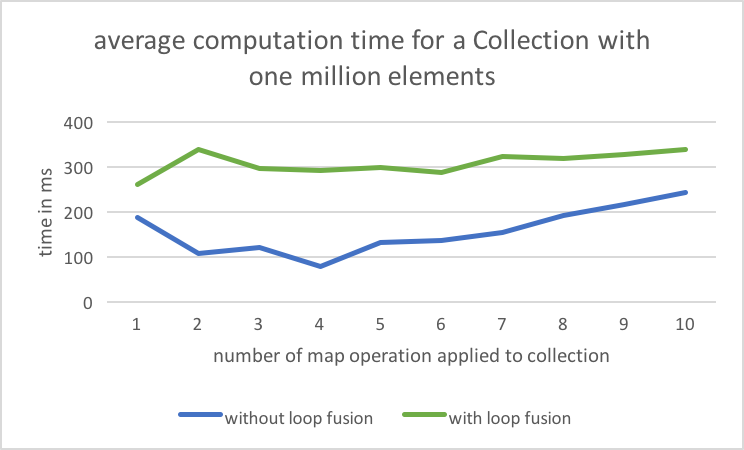
\includegraphics[width=\textwidth]{graphics/million.png}
    \caption{Average compution time for a collection with one million elements.}
    \label{fig:million}
  \end{minipage}
  \hfill
  \begin{minipage}[b]{0.49\textwidth}
    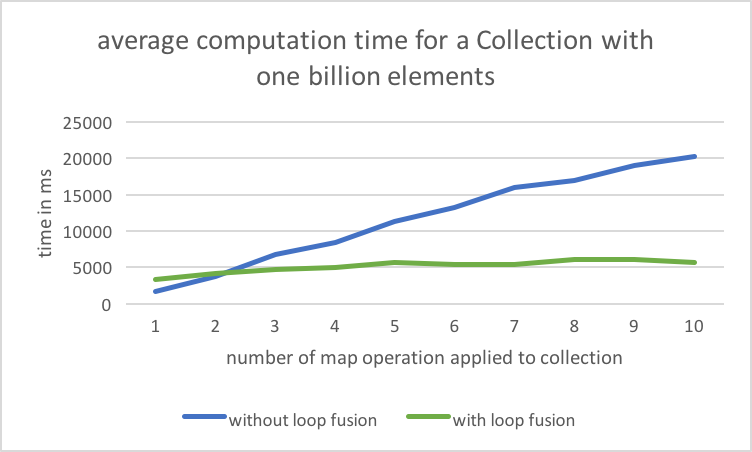
\includegraphics[width=\textwidth]{graphics/billion.png}
    \caption{Average compution time for a collection with ten million elements.}
    \label{fig:ten million}
  \end{minipage}
\end{figure}
\\
For collections with a size of ten million the computation with loop-fusing is most of the time faster than without loop-fusing.
If you apply two maps it is nearly as fast as without fusing and if you apply more than than two maps it gets faster as you can see in Figure~\ref{fig:ten million}.
So starting from collections with a size around ten million loop fusing is an performance boost to mapping over and filter collections.\\
\\
We expected that there would be an performance boost already for collections with a smaller size since it just makes one loop out of many.
But it is needed to add pointcuts for methods which reference to or mutate the collection as described in Section~\ref{sub:applying-ops}.
The advice connected to the join points described by this pointcut seem to slow down the overall computation of the maps.

%%%%%%%%%%%%%%%%%%%%%%%%%%%%%%%%%%%%%%%%%%%%%%%%%%%%%%%%%%%%%%%%%%%%%%%%%%%%%%%
\section{Related Work}\label{sec:related-work}
%%%%%%%%%%%%%%%%%%%%%%%%%%%%%%%%%%%%%%%%%%%%%%%%%%%%%%%%%%%%%%%%%%%%%%%%%%%%%%%

\subsection{Performance Optimized Image Proccesing System with AOP}
One of the early examples of aspect-oriented programming is the Reverse graphics image processing system. The original implementation was an OOP library written in LISP.
A team from Xerox PARC developed an AOP based solution, to overcome performance problems while keeping the understandability and reusability of the OOP solution~\cite{mendhekar1997rg}.\\
They declared three cross-cutting concerns of the system.
The system consists of some base image filters which can be combined to high-level filters, like edge detection.
This is similiar to the map and filter approach presented in this paper and to the general collection method approach.
One cross-cutting concern they specified was the same problem as the one presented in this paper. Each base filter consists of its own loop and the loops accumulate if you use high level filters.
Therefore they invented also a loop fusing aspect. The difference of this approach is that they fused the loops at compile time, which is not possible with AspectJ~\cite{mendhekar1997rg}.

\subsection{Java 8 Streams}
Java 8 introduced the concept of streams. The concept of a stream is different to the one of a collection.
Collections have well defined size and content. Streams are an abstraction of a dataflow. They can be infinite or based on a collection.
They do not base on the principle of iterating over a collection but working on single elements streaming through them.\\
Nevertheless, some features are quite similiar to the solution presented in this paper.
They offer the collection methods in the same way as the Collection class presented in Section~\ref{sub:collection-class}.
Futhermore, they apply the operation in a lazy way, the operations are only applied if there is a consumer for the stream~\cite{java8streams}.
\\

% \subsection{Joins in database management systems} \label{sub:joins}
% Hast du dir schon mal was zu Anfrageplanung bzw. -optimierung in Datenbanksystemen angeschaut? Dort müssen auch (deklarative) SQL-Anfragen umgebaut werden, damit sie performant ausgeführt werden können. Das beinhalten u.a. JOINs was deinen Schleifen ähnelt.

%%%%%%%%%%%%%%%%%%%%%%%%%%%%%%%%%%%%%%%%%%%%%%%%%%%%%%%%%%%%%%%%%%%%%%%%%%%%%%%
\section{Future Work}\label{sec:future-work}
\subsection{Parallel Execution of Operations with Aspects}\label{sub:parallel-execution}
One could use the loop abstraction from the for-loops with operations like map or filter to parallelize their execution.
You could add a layer between these abstraction levels which handles the parallelization concern. Another solution would be to add this ability with an aspect.
In this way the original implementation does not change and you can easily add and remove this aspect as you want to.\\
\\
This could be implemented with an aspect which stops a call to a operation and splits the collection and calls the operation with each fragment. Afterwards it merges all fragments and returns them.

\subsection{Generalized Aspect Compatible to Any Kind of Collection}\label{sub:generalize}
The solution in this paper uses a self-build collection class which can only hold integers and the aspect is specific for this class.
The next step is to generalize this solution. One possible way would be to build a collection class with a generic type and an aspect which could handle that.
Another way could be to build an aspect based on an collection interface so it could be applied to any collection which implements this interface.

%%%%%%%%%%%%%%%%%%%%%%%%%%%%%%%%%%%%%%%%%%%%%%%%%%%%%%%%%%%%%%%%%%%%%%%%%%%%%%%
\section{Conclusion}\label{sec:conclusion}
%%%%%%%%%%%%%%%%%%%%%%%%%%%%%%%%%%%%%%%%%%%%%%%%%%%%%%%%%%%%%%%%%%%%%%%%%%%%%%%
The goal of the loop fusing with aspects was to gain a performance boost without loosing the reusability and readability of the collection methods.
Since the implementation of the collection methods was not changed by the aspect implementation, the second goal was reached.\\
\\
The performance benchmark presented in Section~\ref{sec:performance-comparison} shows that loop fusing can increase the performance of the program.
However, this is just the case for really large collection of the size of ten million. It is a problem that the loop fusing solution is slower for collections smaller than ten million.
So a developer needs to take care about if he applies this aspect or not. This was not intended while developing this solution.\\
\\
One could also merge the anonymous function before passing them to the operations. In this way there cannot be any overhead while executing the loops thus it would be faster to execute.
If you want to reuse your combined anonymous functions you could store them as static methods, so they are globally accessable.
The only issue would be that the developer need to care and think about what to fuse to have a good performance. This is an advantage of the aspect solution where the developer do not need to care about that.

%%%%%%%%%%%%%%%%%%%%%%%%%%%%%%%%%%%%%%%%%%%%%%%%%%%%%%%%%%%%%%%%%%%%%%%%%%%%%%%
\bibliographystyle{splncs03}
\bibliography{paper}

All links were last followed on July 30, 2015.
%%%%%%%%%%%%%%%%%%%%%%%%%%%%%%%%%%%%%%%%%%%%%%%%%%%%%%%%%%%%%%%%%%%%%%%%%%%%%%%

\end{document}
